\documentclass[1p]{elsarticle_modified}
%\bibliographystyle{elsarticle-num}

%\usepackage[colorlinks]{hyperref}
%\usepackage{abbrmath_seonhwa} %\Abb, \Ascr, \Acal ,\Abf, \Afrak
\usepackage{amsfonts}
\usepackage{amssymb}
\usepackage{amsmath}
\usepackage{amsthm}
\usepackage{scalefnt}
\usepackage{amsbsy}
\usepackage{kotex}
\usepackage{caption}
\usepackage{subfig}
\usepackage{color}
\usepackage{graphicx}
\usepackage{xcolor} %% white, black, red, green, blue, cyan, magenta, yellow
\usepackage{float}
\usepackage{setspace}
\usepackage{hyperref}

\usepackage{tikz}
\usetikzlibrary{arrows}

\usepackage{multirow}
\usepackage{array} % fixed length table
\usepackage{hhline}

%%%%%%%%%%%%%%%%%%%%%
\makeatletter
\renewcommand*\env@matrix[1][\arraystretch]{%
	\edef\arraystretch{#1}%
	\hskip -\arraycolsep
	\let\@ifnextchar\new@ifnextchar
	\array{*\c@MaxMatrixCols c}}
\makeatother %https://tex.stackexchange.com/questions/14071/how-can-i-increase-the-line-spacing-in-a-matrix
%%%%%%%%%%%%%%%

\usepackage[normalem]{ulem}

\newcommand{\msout}[1]{\ifmmode\text{\sout{\ensuremath{#1}}}\else\sout{#1}\fi}
%SOURCE: \msout is \stkout macro in https://tex.stackexchange.com/questions/20609/strikeout-in-math-mode

\newcommand{\cancel}[1]{
	\ifmmode
	{\color{red}\msout{#1}}
	\else
	{\color{red}\sout{#1}}
	\fi
}

\newcommand{\add}[1]{
	{\color{blue}\uwave{#1}}
}

\newcommand{\replace}[2]{
	\ifmmode
	{\color{red}\msout{#1}}{\color{blue}\uwave{#2}}
	\else
	{\color{red}\sout{#1}}{\color{blue}\uwave{#2}}
	\fi
}

\newcommand{\Sol}{\mathcal{S}} %segment
\newcommand{\D}{D} %diagram
\newcommand{\A}{\mathcal{A}} %arc


%%%%%%%%%%%%%%%%%%%%%%%%%%%%%5 test

\def\sl{\operatorname{\textup{SL}}(2,\Cbb)}
\def\psl{\operatorname{\textup{PSL}}(2,\Cbb)}
\def\quan{\mkern 1mu \triangleright \mkern 1mu}

\theoremstyle{definition}
\newtheorem{thm}{Theorem}[section]
\newtheorem{prop}[thm]{Proposition}
\newtheorem{lem}[thm]{Lemma}
\newtheorem{ques}[thm]{Question}
\newtheorem{cor}[thm]{Corollary}
\newtheorem{defn}[thm]{Definition}
\newtheorem{exam}[thm]{Example}
\newtheorem{rmk}[thm]{Remark}
\newtheorem{alg}[thm]{Algorithm}

\newcommand{\I}{\sqrt{-1}}
\begin{document}

%\begin{frontmatter}
%
%\title{Boundary parabolic representations of knots up to 8 crossings}
%
%%% Group authors per affiliation:
%\author{Yunhi Cho} 
%\address{Department of Mathematics, University of Seoul, Seoul, Korea}
%\ead{yhcho@uos.ac.kr}
%
%
%\author{Seonhwa Kim} %\fnref{s_kim}}
%\address{Center for Geometry and Physics, Institute for Basic Science, Pohang, 37673, Korea}
%\ead{ryeona17@ibs.re.kr}
%
%\author{Hyuk Kim}
%\address{Department of Mathematical Sciences, Seoul National University, Seoul 08826, Korea}
%\ead{hyukkim@snu.ac.kr}
%
%\author{Seokbeom Yoon}
%\address{Department of Mathematical Sciences, Seoul National University, Seoul, 08826,  Korea}
%\ead{sbyoon15@snu.ac.kr}
%
%\begin{abstract}
%We find all boundary parabolic representation of knots up to 8 crossings.
%
%\end{abstract}
%\begin{keyword}
%    \MSC[2010] 57M25 
%\end{keyword}
%
%\end{frontmatter}

%\linenumbers
%\tableofcontents
%
\newcommand\colored[1]{\textcolor{white}{\rule[-0.35ex]{0.8em}{1.4ex}}\kern-0.8em\color{red} #1}%
%\newcommand\colored[1]{\textcolor{white}{ #1}\kern-2.17ex	\textcolor{white}{ #1}\kern-1.81ex	\textcolor{white}{ #1}\kern-2.15ex\color{red}#1	}

{\Large $\underline{12a_{0254}~(K12a_{0254})}$}

\setlength{\tabcolsep}{10pt}
\renewcommand{\arraystretch}{1.6}
\vspace{1cm}\begin{tabular}{m{100pt}>{\centering\arraybackslash}m{274pt}}
\multirow{5}{120pt}{
	\centering
	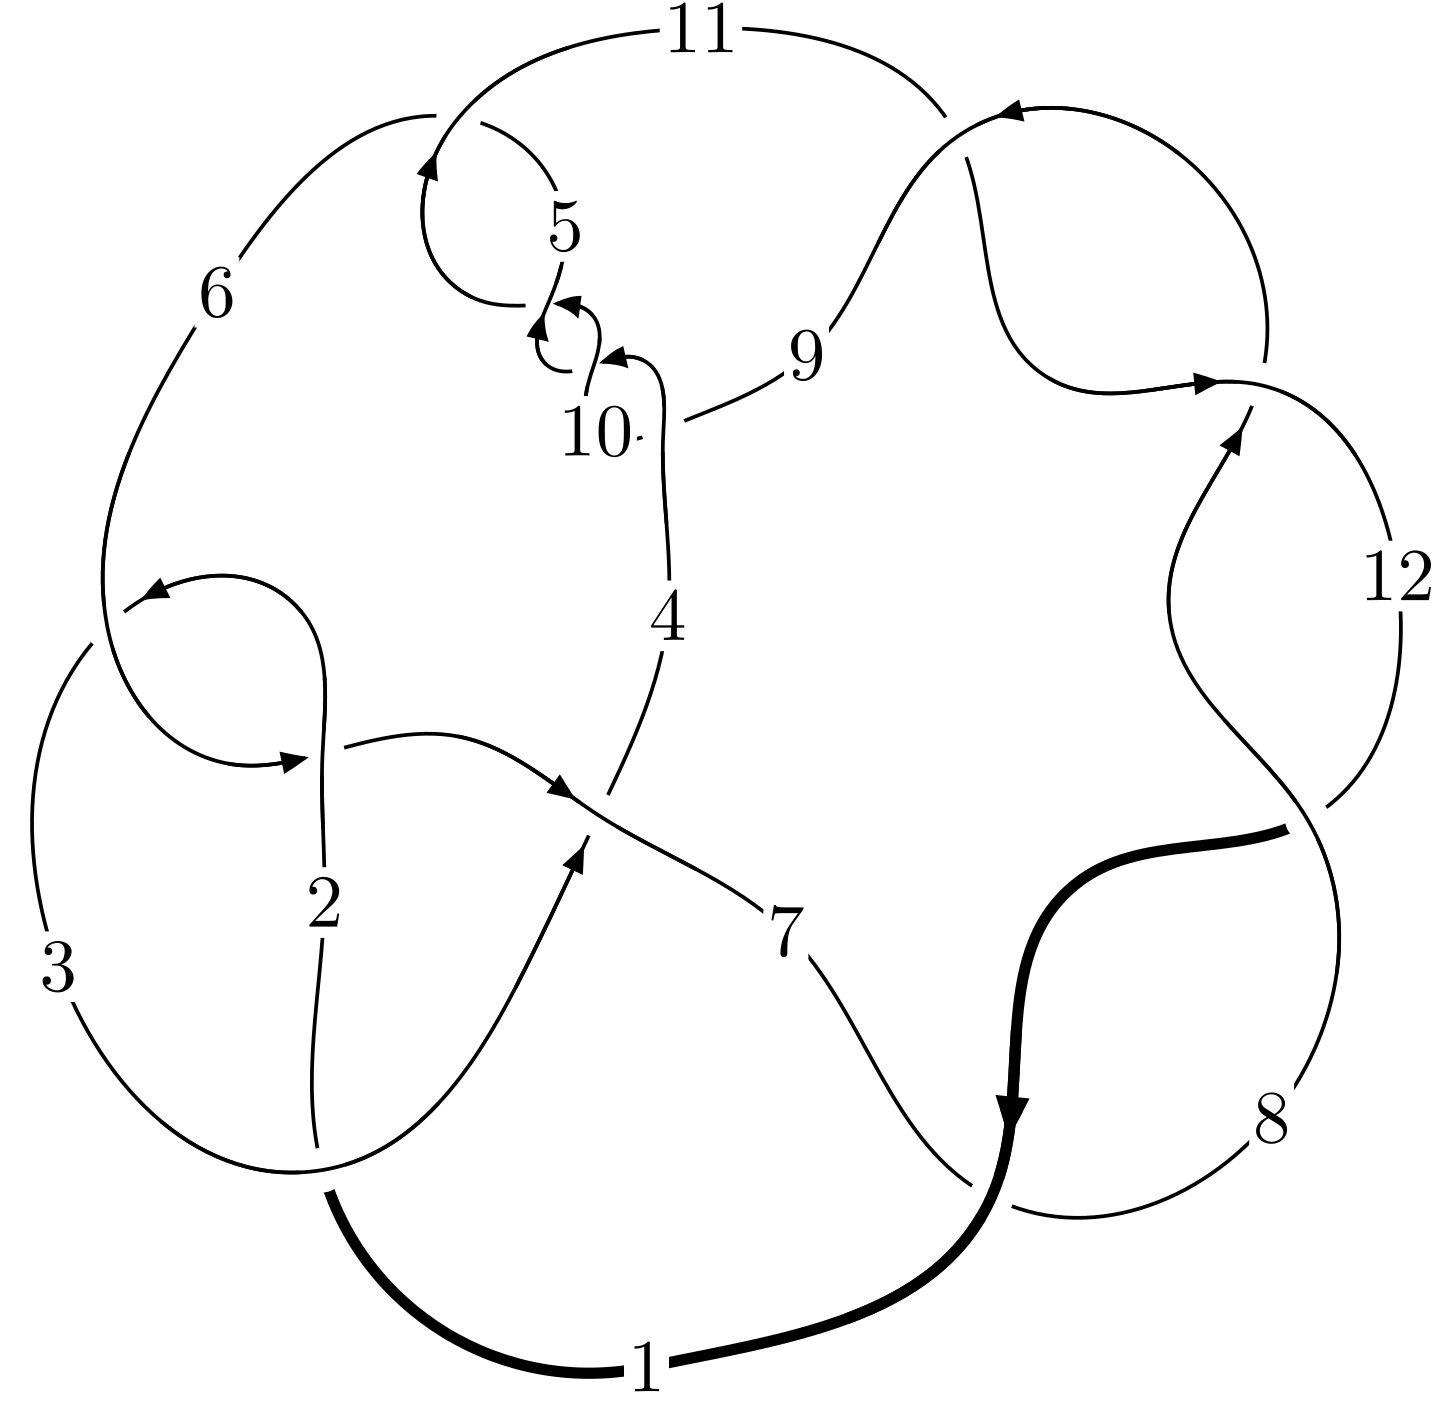
\includegraphics[width=112pt]{../../../GIT/diagram.site/Diagrams/png/1055_12a_0254.png}\\
\ \ \ A knot diagram\footnotemark}&
\allowdisplaybreaks
\textbf{Linearized knot diagam} \\
\cline{2-2}
 &
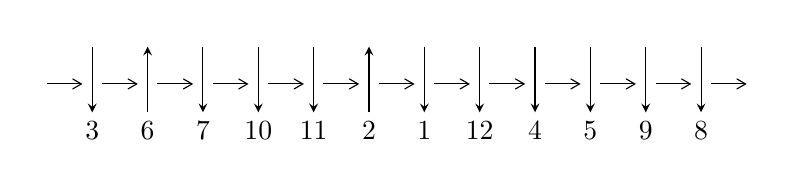
\begin{tikzpicture}[x=20pt, y=17pt]
	% nodes
	\node (C0) at (0, 0) {};
	\node (C1) at (1, 0) {};
	\node (C1U) at (1, +1) {};
	\node (C1D) at (1, -1) {3};

	\node (C2) at (2, 0) {};
	\node (C2U) at (2, +1) {};
	\node (C2D) at (2, -1) {6};

	\node (C3) at (3, 0) {};
	\node (C3U) at (3, +1) {};
	\node (C3D) at (3, -1) {7};

	\node (C4) at (4, 0) {};
	\node (C4U) at (4, +1) {};
	\node (C4D) at (4, -1) {10};

	\node (C5) at (5, 0) {};
	\node (C5U) at (5, +1) {};
	\node (C5D) at (5, -1) {11};

	\node (C6) at (6, 0) {};
	\node (C6U) at (6, +1) {};
	\node (C6D) at (6, -1) {2};

	\node (C7) at (7, 0) {};
	\node (C7U) at (7, +1) {};
	\node (C7D) at (7, -1) {1};

	\node (C8) at (8, 0) {};
	\node (C8U) at (8, +1) {};
	\node (C8D) at (8, -1) {12};

	\node (C9) at (9, 0) {};
	\node (C9U) at (9, +1) {};
	\node (C9D) at (9, -1) {4};

	\node (C10) at (10, 0) {};
	\node (C10U) at (10, +1) {};
	\node (C10D) at (10, -1) {5};

	\node (C11) at (11, 0) {};
	\node (C11U) at (11, +1) {};
	\node (C11D) at (11, -1) {9};

	\node (C12) at (12, 0) {};
	\node (C12U) at (12, +1) {};
	\node (C12D) at (12, -1) {8};
	\node (C13) at (13, 0) {};

	% arrows
	\draw[->,>={angle 60}]
	(C0) edge (C1) (C1) edge (C2) (C2) edge (C3) (C3) edge (C4) (C4) edge (C5) (C5) edge (C6) (C6) edge (C7) (C7) edge (C8) (C8) edge (C9) (C9) edge (C10) (C10) edge (C11) (C11) edge (C12) (C12) edge (C13) ;	\draw[->,>=stealth]
	(C1U) edge (C1D) (C2D) edge (C2U) (C3U) edge (C3D) (C4U) edge (C4D) (C5U) edge (C5D) (C6D) edge (C6U) (C7U) edge (C7D) (C8U) edge (C8D) (C9U) edge (C9D) (C10U) edge (C10D) (C11U) edge (C11D) (C12U) edge (C12D) ;
	\end{tikzpicture} \\
\hhline{~~} \\& 
\textbf{Solving Sequence} \\ \cline{2-2} 
 &
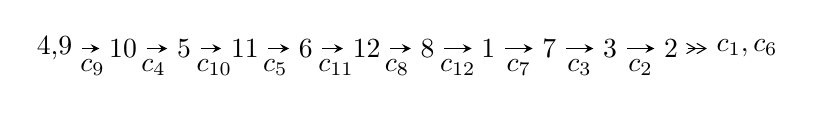
\begin{tikzpicture}[x=22pt, y=7pt]
	% node
	\node (A0) at (-1/8, 0) {4,9};
	\node (A1) at (1, 0) {10};
	\node (A2) at (2, 0) {5};
	\node (A3) at (3, 0) {11};
	\node (A4) at (4, 0) {6};
	\node (A5) at (5, 0) {12};
	\node (A6) at (6, 0) {8};
	\node (A7) at (7, 0) {1};
	\node (A8) at (8, 0) {7};
	\node (A9) at (9, 0) {3};
	\node (A10) at (10, 0) {2};
	\node (C1) at (1/2, -1) {$c_{9}$};
	\node (C2) at (3/2, -1) {$c_{4}$};
	\node (C3) at (5/2, -1) {$c_{10}$};
	\node (C4) at (7/2, -1) {$c_{5}$};
	\node (C5) at (9/2, -1) {$c_{11}$};
	\node (C6) at (11/2, -1) {$c_{8}$};
	\node (C7) at (13/2, -1) {$c_{12}$};
	\node (C8) at (15/2, -1) {$c_{7}$};
	\node (C9) at (17/2, -1) {$c_{3}$};
	\node (C10) at (19/2, -1) {$c_{2}$};
	\node (A11) at (45/4, 0) {$c_{1},c_{6}$};

	% edge
	\draw[->,>=stealth]	
	(A0) edge (A1) (A1) edge (A2) (A2) edge (A3) (A3) edge (A4) (A4) edge (A5) (A5) edge (A6) (A6) edge (A7) (A7) edge (A8) (A8) edge (A9) (A9) edge (A10) ;
	\draw[->>,>={angle 60}]	
	(A10) edge (A11);
\end{tikzpicture} \\ 

\end{tabular} \\

\footnotetext{
The image of knot diagram is generated by the software ``\textbf{Draw programme}" developed by Andrew Bartholomew(\url{http://www.layer8.co.uk/maths/draw/index.htm\#Running-draw}), where we modified some parts for our purpose(\url{https://github.com/CATsTAILs/LinksPainter}).
}\phantom \\ \newline 
\centering \textbf{Ideals for irreducible components\footnotemark of $X_{\text{par}}$} 
 
\begin{align*}
I^u_{1}&=\langle 
u^{48}- u^{47}+\cdots+2 u-1\rangle \\
\\
\end{align*}
\raggedright * 1 irreducible components of $\dim_{\mathbb{C}}=0$, with total 48 representations.\\
\footnotetext{All coefficients of polynomials are rational numbers. But the coefficients are sometimes approximated in decimal forms when there is not enough margin.}
\newpage
\renewcommand{\arraystretch}{1}
\centering \section*{I. $I^u_{1}= \langle u^{48}- u^{47}+\cdots+2 u-1 \rangle$}
\flushleft \textbf{(i) Arc colorings}\\
\begin{tabular}{m{7pt} m{180pt} m{7pt} m{180pt} }
\flushright $a_{4}=$&$\begin{pmatrix}0\\u\end{pmatrix}$ \\
\flushright $a_{9}=$&$\begin{pmatrix}1\\0\end{pmatrix}$ \\
\flushright $a_{10}=$&$\begin{pmatrix}1\\u^2\end{pmatrix}$ \\
\flushright $a_{5}=$&$\begin{pmatrix}- u\\- u^3+u\end{pmatrix}$ \\
\flushright $a_{11}=$&$\begin{pmatrix}- u^2+1\\- u^4+2 u^2\end{pmatrix}$ \\
\flushright $a_{6}=$&$\begin{pmatrix}u^3-2 u\\u^5-3 u^3+u\end{pmatrix}$ \\
\flushright $a_{12}=$&$\begin{pmatrix}u^4-3 u^2+1\\- u^4+2 u^2\end{pmatrix}$ \\
\flushright $a_{8}=$&$\begin{pmatrix}u^8-5 u^6+7 u^4-2 u^2+1\\- u^8+4 u^6-4 u^4\end{pmatrix}$ \\
\flushright $a_{1}=$&$\begin{pmatrix}u^{12}-7 u^{10}+17 u^8-16 u^6+6 u^4-5 u^2+1\\- u^{12}+6 u^{10}-12 u^8+8 u^6- u^4+2 u^2\end{pmatrix}$ \\
\flushright $a_{7}=$&$\begin{pmatrix}u^{16}-9 u^{14}+31 u^{12}-50 u^{10}+39 u^8-22 u^6+18 u^4-4 u^2+1\\- u^{16}+8 u^{14}-24 u^{12}+32 u^{10}-18 u^8+8 u^6-8 u^4\end{pmatrix}$ \\
\flushright $a_{3}=$&$\begin{pmatrix}u^{33}-18 u^{31}+\cdots-8 u^3+u\\- u^{33}+17 u^{31}+\cdots-8 u^5+u\end{pmatrix}$ \\
\flushright $a_{2}=$&$\begin{pmatrix}u^{41}-22 u^{39}+\cdots-14 u^3+u\\u^{43}-23 u^{41}+\cdots+3 u^3+u\end{pmatrix}$\\&\end{tabular}
\flushleft \textbf{(ii) Obstruction class $= -1$}\\~\\
\flushleft \textbf{(iii) Cusp Shapes $= 4 u^{45}-96 u^{43}+\cdots+8 u-14$}\\~\\
\newpage\renewcommand{\arraystretch}{1}
\flushleft \textbf{(iv) u-Polynomials at the component}\newline \\
\begin{tabular}{m{50pt}|m{274pt}}
Crossings & \hspace{64pt}u-Polynomials at each crossing \\
\hline $$\begin{aligned}c_{1}\end{aligned}$$&$\begin{aligned}
&u^{48}+21 u^{47}+\cdots-4 u+1
\end{aligned}$\\
\hline $$\begin{aligned}c_{2},c_{6}\end{aligned}$$&$\begin{aligned}
&u^{48}- u^{47}+\cdots+2 u^2-1
\end{aligned}$\\
\hline $$\begin{aligned}c_{3}\end{aligned}$$&$\begin{aligned}
&u^{48}+u^{47}+\cdots-18 u-5
\end{aligned}$\\
\hline $$\begin{aligned}c_{4},c_{5},c_{9}\\c_{10}\end{aligned}$$&$\begin{aligned}
&u^{48}+u^{47}+\cdots-2 u-1
\end{aligned}$\\
\hline $$\begin{aligned}c_{7},c_{8},c_{11}\\c_{12}\end{aligned}$$&$\begin{aligned}
&u^{48}-5 u^{47}+\cdots+40 u-7
\end{aligned}$\\
\hline
\end{tabular}\\~\\
\newpage\renewcommand{\arraystretch}{1}
\flushleft \textbf{(v) Riley Polynomials at the component}\newline \\
\begin{tabular}{m{50pt}|m{274pt}}
Crossings & \hspace{64pt}Riley Polynomials at each crossing \\
\hline $$\begin{aligned}c_{1}\end{aligned}$$&$\begin{aligned}
&y^{48}+13 y^{47}+\cdots-64 y+1
\end{aligned}$\\
\hline $$\begin{aligned}c_{2},c_{6}\end{aligned}$$&$\begin{aligned}
&y^{48}+21 y^{47}+\cdots-4 y+1
\end{aligned}$\\
\hline $$\begin{aligned}c_{3}\end{aligned}$$&$\begin{aligned}
&y^{48}+5 y^{47}+\cdots+436 y+25
\end{aligned}$\\
\hline $$\begin{aligned}c_{4},c_{5},c_{9}\\c_{10}\end{aligned}$$&$\begin{aligned}
&y^{48}-51 y^{47}+\cdots-4 y+1
\end{aligned}$\\
\hline $$\begin{aligned}c_{7},c_{8},c_{11}\\c_{12}\end{aligned}$$&$\begin{aligned}
&y^{48}+57 y^{47}+\cdots+360 y+49
\end{aligned}$\\
\hline
\end{tabular}\\~\\
\newpage\flushleft \textbf{(vi) Complex Volumes and Cusp Shapes}
$$\begin{array}{c|c|c}  
\text{Solutions to }I^u_{1}& \I (\text{vol} + \sqrt{-1}CS) & \text{Cusp shape}\\
 \hline 
\begin{aligned}
u &= -0.531007 + 0.671464 I\end{aligned}
 & \phantom{-}9.01669 + 9.40336 I & -5.02805 - 7.67988 I \\ \hline\begin{aligned}
u &= -0.531007 - 0.671464 I\end{aligned}
 & \phantom{-}9.01669 - 9.40336 I & -5.02805 + 7.67988 I \\ \hline\begin{aligned}
u &= \phantom{-}0.521293 + 0.674135 I\end{aligned}
 & \phantom{-}10.82160 - 3.97968 I & -2.45267 + 3.13488 I \\ \hline\begin{aligned}
u &= \phantom{-}0.521293 - 0.674135 I\end{aligned}
 & \phantom{-}10.82160 + 3.97968 I & -2.45267 - 3.13488 I \\ \hline\begin{aligned}
u &= \phantom{-}0.496510 + 0.679990 I\end{aligned}
 & \phantom{-}10.89560 - 0.56946 I & -2.23785 + 2.73831 I \\ \hline\begin{aligned}
u &= \phantom{-}0.496510 - 0.679990 I\end{aligned}
 & \phantom{-}10.89560 + 0.56946 I & -2.23785 - 2.73831 I \\ \hline\begin{aligned}
u &= -0.485958 + 0.681983 I\end{aligned}
 & \phantom{-}9.15118 - 4.85655 I & -4.61319 + 1.88995 I \\ \hline\begin{aligned}
u &= -0.485958 - 0.681983 I\end{aligned}
 & \phantom{-}9.15118 + 4.85655 I & -4.61319 - 1.88995 I \\ \hline\begin{aligned}
u &= -0.504951 + 0.655491 I\end{aligned}
 & \phantom{-}5.09552 + 2.21064 I & -8.17139 - 3.04652 I \\ \hline\begin{aligned}
u &= -0.504951 - 0.655491 I\end{aligned}
 & \phantom{-}5.09552 - 2.21064 I & -8.17139 + 3.04652 I \\ \hline\begin{aligned}
u &= \phantom{-}0.565305 + 0.449893 I\end{aligned}
 & \phantom{-}0.20947 - 6.94753 I & -8.17814 + 10.14161 I \\ \hline\begin{aligned}
u &= \phantom{-}0.565305 - 0.449893 I\end{aligned}
 & \phantom{-}0.20947 + 6.94753 I & -8.17814 - 10.14161 I \\ \hline\begin{aligned}
u &= -0.507179 + 0.452333 I\end{aligned}
 & \phantom{-}2.02075 + 2.34431 I & -3.97357 - 5.45884 I \\ \hline\begin{aligned}
u &= -0.507179 - 0.452333 I\end{aligned}
 & \phantom{-}2.02075 - 2.34431 I & -3.97357 + 5.45884 I \\ \hline\begin{aligned}
u &= -0.639814 + 0.094545 I\end{aligned}
 & -2.90001 + 3.13118 I & -15.9591 - 5.8893 I \\ \hline\begin{aligned}
u &= -0.639814 - 0.094545 I\end{aligned}
 & -2.90001 - 3.13118 I & -15.9591 + 5.8893 I \\ \hline\begin{aligned}
u &= \phantom{-}0.547494 + 0.306761 I\end{aligned}
 & -1.75783 - 0.64590 I & -12.93673 + 4.70290 I \\ \hline\begin{aligned}
u &= \phantom{-}0.547494 - 0.306761 I\end{aligned}
 & -1.75783 + 0.64590 I & -12.93673 - 4.70290 I \\ \hline\begin{aligned}
u &= -0.376501 + 0.479727 I\end{aligned}
 & \phantom{-}2.41689 + 0.90085 I & -1.85528 - 3.88194 I \\ \hline\begin{aligned}
u &= -0.376501 - 0.479727 I\end{aligned}
 & \phantom{-}2.41689 - 0.90085 I & -1.85528 + 3.88194 I \\ \hline\begin{aligned}
u &= \phantom{-}0.303476 + 0.502707 I\end{aligned}
 & \phantom{-}0.99759 + 3.64557 I & -4.52853 - 2.54638 I \\ \hline\begin{aligned}
u &= \phantom{-}0.303476 - 0.502707 I\end{aligned}
 & \phantom{-}0.99759 - 3.64557 I & -4.52853 + 2.54638 I \\ \hline\begin{aligned}
u &= -1.43629 + 0.07552 I\end{aligned}
 & -4.47416 - 1.80540 I & \phantom{-0.000000 } 0 \\ \hline\begin{aligned}
u &= -1.43629 - 0.07552 I\end{aligned}
 & -4.47416 + 1.80540 I & \phantom{-0.000000 } 0 \\ \hline\begin{aligned}
u &= \phantom{-}1.46538 + 0.10192 I\end{aligned}
 & -3.55328 - 2.83353 I & \phantom{-0.000000 } 0 \\ \hline\begin{aligned}
u &= \phantom{-}1.46538 - 0.10192 I\end{aligned}
 & -3.55328 + 2.83353 I & \phantom{-0.000000 } 0 \\ \hline\begin{aligned}
u &= \phantom{-}1.49909 + 0.21897 I\end{aligned}
 & \phantom{-}2.68595 + 1.60072 I & \phantom{-0.000000 } 0 \\ \hline\begin{aligned}
u &= \phantom{-}1.49909 - 0.21897 I\end{aligned}
 & \phantom{-}2.68595 - 1.60072 I & \phantom{-0.000000 } 0 \\ \hline\begin{aligned}
u &= -1.50624 + 0.21870 I\end{aligned}
 & \phantom{-}4.35978 + 3.82234 I & \phantom{-0.000000 } 0 \\ \hline\begin{aligned}
u &= -1.50624 - 0.21870 I\end{aligned}
 & \phantom{-}4.35978 - 3.82234 I & \phantom{-0.000000 } 0\\
 \hline 
 \end{array}$$\newpage$$\begin{array}{c|c|c}  
\text{Solutions to }I^u_{1}& \I (\text{vol} + \sqrt{-1}CS) & \text{Cusp shape}\\
 \hline 
\begin{aligned}
u &= \phantom{-}1.51915 + 0.11525 I\end{aligned}
 & -4.70339 - 4.31197 I & \phantom{-0.000000 } 0 \\ \hline\begin{aligned}
u &= \phantom{-}1.51915 - 0.11525 I\end{aligned}
 & -4.70339 + 4.31197 I & \phantom{-0.000000 } 0 \\ \hline\begin{aligned}
u &= -1.52354\phantom{ +0.000000I}\end{aligned}
 & -7.47236\phantom{ +0.000000I} & \phantom{-0.000000 } 0 \\ \hline\begin{aligned}
u &= \phantom{-}1.51456 + 0.20489 I\end{aligned}
 & -1.52188 - 5.31834 I & \phantom{-0.000000 } 0 \\ \hline\begin{aligned}
u &= \phantom{-}1.51456 - 0.20489 I\end{aligned}
 & -1.52188 + 5.31834 I & \phantom{-0.000000 } 0 \\ \hline\begin{aligned}
u &= \phantom{-}0.466355\phantom{ +0.000000I}\end{aligned}
 & -0.719382\phantom{ +0.000000I} & -13.6590\phantom{ +0.000000I} \\ \hline\begin{aligned}
u &= -1.53316 + 0.08163 I\end{aligned}
 & -8.71798 + 2.01778 I & \phantom{-0.000000 } 0 \\ \hline\begin{aligned}
u &= -1.53316 - 0.08163 I\end{aligned}
 & -8.71798 - 2.01778 I & \phantom{-0.000000 } 0 \\ \hline\begin{aligned}
u &= -1.52160 + 0.21684 I\end{aligned}
 & \phantom{-}4.12565 + 7.21700 I & \phantom{-0.000000 } 0 \\ \hline\begin{aligned}
u &= -1.52160 - 0.21684 I\end{aligned}
 & \phantom{-}4.12565 - 7.21700 I & \phantom{-0.000000 } 0 \\ \hline\begin{aligned}
u &= \phantom{-}1.52715 + 0.21588 I\end{aligned}
 & \phantom{-}2.25992 - 12.63260 I & \phantom{-0.000000 } 0 \\ \hline\begin{aligned}
u &= \phantom{-}1.52715 - 0.21588 I\end{aligned}
 & \phantom{-}2.25992 + 12.63260 I & \phantom{-0.000000 } 0 \\ \hline\begin{aligned}
u &= -1.53825 + 0.11928 I\end{aligned}
 & -6.80498 + 8.95605 I & \phantom{-0.000000 } 0 \\ \hline\begin{aligned}
u &= -1.53825 - 0.11928 I\end{aligned}
 & -6.80498 - 8.95605 I & \phantom{-0.000000 } 0 \\ \hline\begin{aligned}
u &= \phantom{-}1.54951 + 0.01876 I\end{aligned}
 & -10.22470 - 3.49526 I & \phantom{-0.000000 } 0 \\ \hline\begin{aligned}
u &= \phantom{-}1.54951 - 0.01876 I\end{aligned}
 & -10.22470 + 3.49526 I & \phantom{-0.000000 } 0 \\ \hline\begin{aligned}
u &= \phantom{-}0.100637 + 0.382710 I\end{aligned}
 & -0.49816 - 1.64037 I & -4.69035 + 3.89080 I \\ \hline\begin{aligned}
u &= \phantom{-}0.100637 - 0.382710 I\end{aligned}
 & -0.49816 + 1.64037 I & -4.69035 - 3.89080 I\\
 \hline 
 \end{array}$$\newpage
\newpage\renewcommand{\arraystretch}{1}
\centering \section*{ II. u-Polynomials}
\begin{tabular}{m{50pt}|m{274pt}}
Crossings & \hspace{64pt}u-Polynomials at each crossing \\
\hline $$\begin{aligned}c_{1}\end{aligned}$$&$\begin{aligned}
&u^{48}+21 u^{47}+\cdots-4 u+1
\end{aligned}$\\
\hline $$\begin{aligned}c_{2},c_{6}\end{aligned}$$&$\begin{aligned}
&u^{48}- u^{47}+\cdots+2 u^2-1
\end{aligned}$\\
\hline $$\begin{aligned}c_{3}\end{aligned}$$&$\begin{aligned}
&u^{48}+u^{47}+\cdots-18 u-5
\end{aligned}$\\
\hline $$\begin{aligned}c_{4},c_{5},c_{9}\\c_{10}\end{aligned}$$&$\begin{aligned}
&u^{48}+u^{47}+\cdots-2 u-1
\end{aligned}$\\
\hline $$\begin{aligned}c_{7},c_{8},c_{11}\\c_{12}\end{aligned}$$&$\begin{aligned}
&u^{48}-5 u^{47}+\cdots+40 u-7
\end{aligned}$\\
\hline
\end{tabular}\newpage\renewcommand{\arraystretch}{1}
\centering \section*{ III. Riley Polynomials}
\begin{tabular}{m{50pt}|m{274pt}}
Crossings & \hspace{64pt}Riley Polynomials at each crossing \\
\hline $$\begin{aligned}c_{1}\end{aligned}$$&$\begin{aligned}
&y^{48}+13 y^{47}+\cdots-64 y+1
\end{aligned}$\\
\hline $$\begin{aligned}c_{2},c_{6}\end{aligned}$$&$\begin{aligned}
&y^{48}+21 y^{47}+\cdots-4 y+1
\end{aligned}$\\
\hline $$\begin{aligned}c_{3}\end{aligned}$$&$\begin{aligned}
&y^{48}+5 y^{47}+\cdots+436 y+25
\end{aligned}$\\
\hline $$\begin{aligned}c_{4},c_{5},c_{9}\\c_{10}\end{aligned}$$&$\begin{aligned}
&y^{48}-51 y^{47}+\cdots-4 y+1
\end{aligned}$\\
\hline $$\begin{aligned}c_{7},c_{8},c_{11}\\c_{12}\end{aligned}$$&$\begin{aligned}
&y^{48}+57 y^{47}+\cdots+360 y+49
\end{aligned}$\\
\hline
\end{tabular}
\vskip 2pc
\end{document}